% ============================================================
% Capítulo: Declaraciones (Bloque B.15)
% ============================================================
\chapter{Declaraciones}

Este capítulo reúne las declaraciones formales que la guía exige antes de
las referencias bibliográficas. Sigue el mismo criterio de honestidad
metodológica que el resto del documento: los datos verificables en el
propio repositorio se presentan como tales, y los que exigen una
decisión que solo puede tomar el equipo (financiamiento, conflictos de
interés, distribución exacta de contribuciones) se dejan marcados de
forma explícita como pendientes, en vez de decidirse unilateralmente en
este documento.

\section{Disponibilidad de código}
\label{sec:decl-codigo}

El código fuente completo de SGB-SaaS (backend Spring Boot, frontend
Angular, scripts de medición, infraestructura Docker) está disponible
públicamente bajo licencia MIT (\texttt{LICENSE}, raíz del repositorio)
en:

\begin{center}
\url{https://github.com/mloorm14/sgb-saas}
\end{center}

El software citable de esta entrega corresponde al commit etiquetado
como \texttt{v1.0.0} (resoluble con \texttt{git rev-list -n 1 v1.0.0};
ver portada de este documento). Los metadatos de citación siguen el
formato Citation File Format 1.2.0 (\texttt{CITATION.cff}, raíz del
repositorio), con ORCID verificado de los 3 autores.

\section{Disponibilidad de datos}

Los datos empíricos crudos que sustentan el \autoref{cap:resultados}
(salidas de k6, reportes JaCoCo en XML/CSV/HTML, resultados de
Lighthouse, evidencia de auditoría OWASP control por control) están
versionados junto con el código fuente en \texttt{docs/mediciones/}, en
el mismo repositorio citado en la
\autoref{sec:decl-codigo}. \texttt{LICENSE} cubre el repositorio
completo (\emph{"the Software"}, sin excluir explícitamente los datos de
\texttt{docs/}), por lo que estos datos quedan bajo la misma licencia
MIT que el software -- el equipo no ha declarado hasta la fecha una
licencia de datos separada (p.~ej.\ CC-BY) para este material, algo que
podría formalizarse en una futura revisión de \texttt{LICENSE} si el
equipo lo considera necesario.

Este conjunto de datos empíricos \textbf{no cuenta con un DOI propio
independiente} -- el equipo decidió no crear un archivado separado en
un repositorio de datos (Zenodo permite archivar datasets con su
propio DOI, distinto del DOI del software), y en su lugar lo cubre
bajo el mismo DOI del software citado en la portada de este documento
(\texttt{10.5281/zenodo.22741050}), ya que ambos se versionan juntos
en el mismo repositorio y bajo la misma licencia MIT
(\autoref{sec:decl-codigo}).

Los formularios de consentimiento informado, correos y firmas de la
corrida SUS ejecutada el 19 de septiembre de 2026 permanecen fuera de
este repositorio y de cualquier archivado público. En cambio,
\texttt{docs/mediciones/sus/sus.csv} contiene únicamente las 15 filas
anonimizadas autorizadas para la evaluación académica; el manifiesto por
código permite al docente contrastarlas con los registros privados sin
exponer identidades. El 20 de septiembre de 2026 a las 16:12 se preservó
un export CSV privado del formulario original con 17 registros; su huella
SHA-256 se declara en
\texttt{docs/mediciones/sus/RAW-EXPORT-ATTESTATION.md}. Esta constancia no
sustituye el registro fuente ni lo convierte en dato público: ante
solicitud, el docente puede contrastar en privado al menos tres códigos
del manifiesto con las marcas temporales y respuestas del export original.

\section{Disponibilidad de materiales}

Los instrumentos y materiales usados para producir la evidencia de este
documento están versionados como parte del propio repositorio de
código, no como capturas de pantalla ni archivos externos no
trazables:

\begin{itemize}[leftmargin=1.2cm]
  \item \textbf{Colección de peticiones HTTP}: \texttt{docs/postman/coleccion.json},
    con 66 peticiones reales que cubren los módulos de
    Auth, Libros, Préstamos, Reservaciones, Multas, Configuración,
    Credencial QR, Notificaciones, Usuarios (Admin), Auditoría y
    Chatbot, incluyendo casos de error (401/403/404/422/423/429). Nota
    de honestidad: \texttt{docs/observaciones/OBSERVACIONES.md} (OBS-03)
    registra 39 peticiones como la cifra vigente en el commit
    \texttt{c6b372c} (cierre de la Tercera Entrega); el conteo real
    verificado directamente sobre el archivo actual para este capítulo
    es 66 -- la colección creció junto con los 8 módulos de dominio
    mergeados durante esta entrega, y esa cifra antigua no se actualizó
    en su momento en \texttt{OBSERVACIONES.md}.
  \item \textbf{Scripts de carga (k6)}: \texttt{k6/}, con semilla fija
    documentada (\autoref{sec:mm-semillas}) para reproducibilidad.
  \item \textbf{Script de análisis estadístico}: \texttt{scripts/perf-analysis.py}
    (bootstrap de IC~95\,\% sobre p95, semilla fija \texttt{BOOTSTRAP\_SEED = 42}).
  \item \textbf{Configuración de Lighthouse CI}: \texttt{frontend-angular/lighthouserc.js},
    con el perfil móvil/Slow~4G ya parametrizado y comentado, listo para
    ejecutarse contra el stack Docker real.
  \item \textbf{Evidencia de usabilidad SUS}: instrumento aplicado,
    CSV anónimo de 15 respuestas, manifiesto de consentimientos,
    recálculo y figuras en \texttt{docs/mediciones/sus/}. Las firmas y
    registros identificables permanecen bajo custodia privada.
\end{itemize}

\section{Declaración ética}
\label{sec:decl-etica}

El tratamiento de datos personales y el protocolo de consentimiento
informado para las pruebas de usabilidad SUS están documentados en
detalle en \texttt{docs/etica/ETHICS.md}, verificado directamente para
este capítulo. En síntesis:

\begin{itemize}[leftmargin=1.2cm]
  \item Los datos de ejemplo del sistema (\texttt{db/seed.sql}) usan
    metadatos bibliográficos públicos de libros reales publicados (ISBN,
    título, autor, editorial); ninguna contraseña se almacena en texto
    plano (hash BCrypt, costo 12); se verificó por auditoría de código
    que ningún endpoint expone el campo \texttt{passwordHash}.
  \item Los 15 participantes incluidos en la corrida SUS confirmaron ser
    mayores de edad, aceptaron el consentimiento y firmaron el formulario
    privado. La publicación expone solo códigos P01--P15 y datos
    anonimizados; la custodia permite revisión docente bajo solicitud.
  \item Los formularios originales, firmas y correos \textbf{no se
    suben} a este repositorio público. El manifiesto declara de forma
    transparente que la autorización para publicar las filas anónimas se
    confirmó oralmente el 19 de septiembre de 2026.
\end{itemize}

\section{Contribuciones de autoría (taxonomía CRediT)}

La \autoref{tab:decl-credit} resume la distribución de roles de
autoría por integrante, siguiendo la taxonomía CRediT.

\begin{table}[h]
\centering
\small
\begin{tabular}{@{}p{4.6cm}ccc@{}}
\toprule
\textbf{Rol CRediT} & \textbf{Cajas} & \textbf{Loor} & \textbf{Panamá} \\
\midrule
Conceptualization        & \checkmark & \checkmark & \checkmark \\
Data curation             & \checkmark & \checkmark & \checkmark \\
Formal analysis           &            & \checkmark &            \\
Funding acquisition       & \multicolumn{3}{c}{No aplica -- sin financiamiento externo declarado} \\
Investigation              & \checkmark & \checkmark & \checkmark \\
Methodology                & \checkmark & \checkmark &            \\
Project administration     &            & \checkmark &            \\
Resources                  & \checkmark & \checkmark & \checkmark \\
Software                   & \checkmark & \checkmark & \checkmark \\
Supervision                & \multicolumn{3}{c}{Ver nota debajo de la tabla} \\
Validation                  & \checkmark & \checkmark & \checkmark \\
Visualization               & \checkmark & \checkmark & \checkmark \\
Writing -- original draft    &            & \checkmark &            \\
Writing -- review \& editing  & \checkmark & \checkmark & \checkmark \\
\bottomrule
\end{tabular}
\caption{Distribución de roles CRediT del equipo SGB-SaaS.}
\label{tab:decl-credit}
\end{table}

Justificación de la propuesta, con evidencia concreta verificada para
este capítulo:

\begin{itemize}[leftmargin=1.2cm]
  \item \textbf{Cajas}: autor del mayor volumen de commits del proyecto
    (764 commits humanos sin merges según
    \texttt{git -c log.mailmap=true shortlog -sne --no-merges HEAD} al
    rev \texttt{3489e2c5}; conteos vigentes por rol en
    \texttt{CONTRIBUCIONES.md}),
    concentrados en el backend Spring Boot -- servicios, controladores,
    la validación estricta de \texttt{@Procedure}/
    \texttt{@NamedStoredProcedureQuery} para los procedimientos
    principales (\autoref{cap:discusion}), y la mayoría
    de los tests automatizados del backend. Autor de los 8 módulos
    de dominio mergeados en esta entrega. Asignado también a la
    auditoría ZAP baseline pendiente (\autoref{sec:tf-zap}).
  \item \textbf{Loor}: autor de la mayoría de los commits de
    \texttt{docs/} (este informe, arquitectura C4, ADRs, bibliografía
    verificada contra Crossref), de los scripts de medición
    (\texttt{k6/}, \texttt{scripts/perf-analysis.py}) y del análisis
    estadístico del \autoref{cap:resultados}. 344 commits humanos sin
    merges según la misma consulta con \texttt{.mailmap} (rev
    \texttt{3489e2c5}; conteos vigentes por rol en
    \texttt{CONTRIBUCIONES.md}).
  \item \textbf{Panamá}: autor de los componentes de frontend de
    Préstamos, Reservaciones y Multas (\texttt{frontend-angular/}) y de
    varias historias de usuario en \texttt{docs/requisitos/}. 370 commits humanos sin merges según la misma consulta con
    \texttt{.mailmap} (rev \texttt{3489e2c5}; conteos vigentes por
    rol en \texttt{CONTRIBUCIONES.md}). Ejecutó el cierre SUS de
    $N=15$; sus límites de muestreo y privacidad se documentan en
    \texttt{docs/mediciones/sus/} y \autoref{sec:tf-sus}.
\end{itemize}

La actividad temporal y el reparto por autor se visualizan en las
\autoref{fig:decl-commits-mensuales} y \autoref{fig:decl-commits-autores},
generadas desde \texttt{git log} con
\texttt{scripts/generar-figuras-evaluacion.py} (conteos sin merges,
con \texttt{.mailmap}).

\begin{figure}[h]
\centering
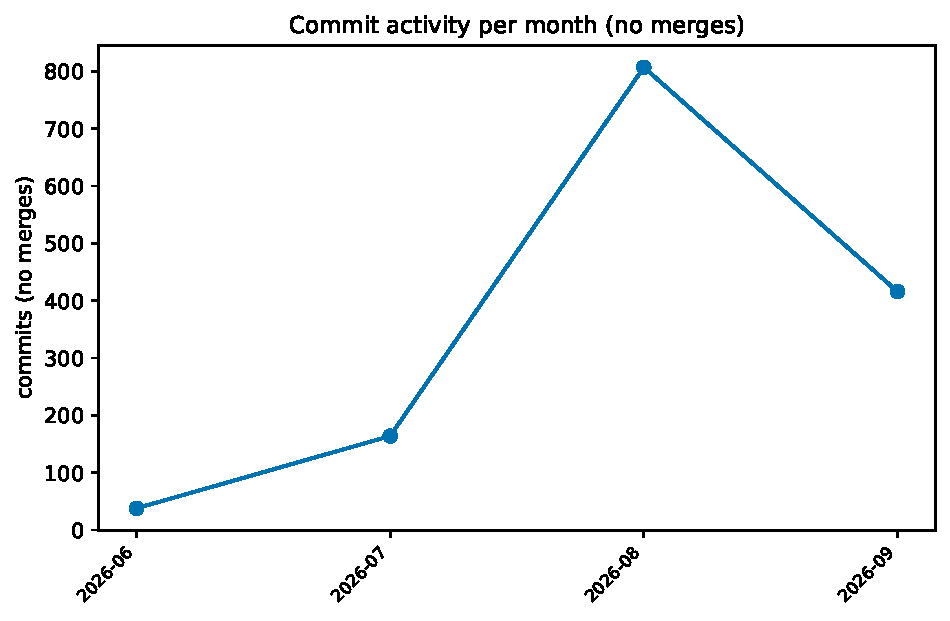
\includegraphics[width=0.85\textwidth]{mediciones/figuras/fig-commits-mensuales.pdf}
\caption{Commit activity per month (no merges). Generated from
\texttt{git log} with
\texttt{scripts/generar-figuras-evaluacion.py}.}
\label{fig:decl-commits-mensuales}
\end{figure}

\begin{figure}[h]
\centering
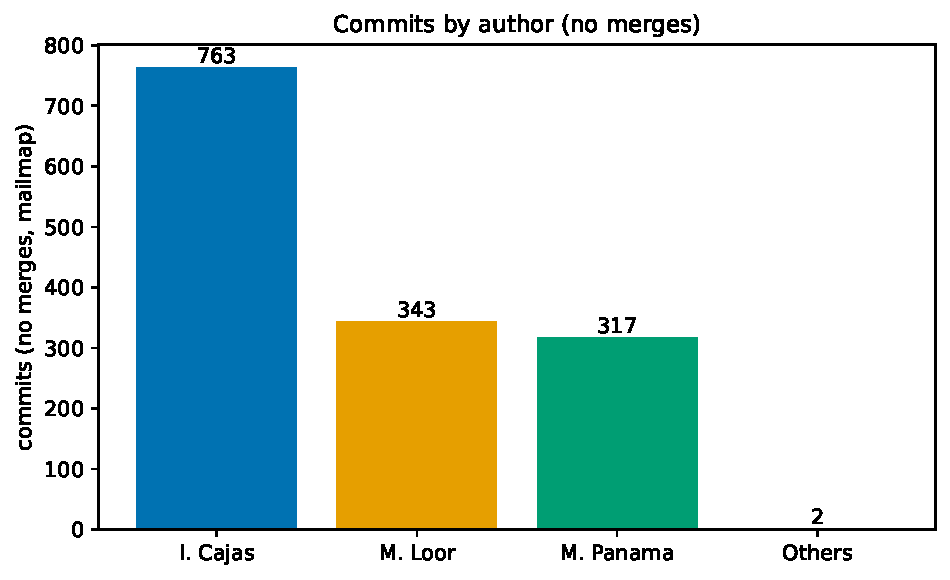
\includegraphics[width=0.7\textwidth]{mediciones/figuras/fig-commits-autores.pdf}
\caption{Commits by author (no merges, identities unified with
\texttt{.mailmap}). Generated from \texttt{git shortlog} with
\texttt{scripts/generar-figuras-evaluacion.py}.}
\label{fig:decl-commits-autores}
\end{figure}

\textbf{Nota sobre "Supervision".} La guía CRediT reserva este rol
típicamente para quien dirige el trabajo sin ser autor operativo directo
del código -- en este PFC, ese rol lo ejerce el docente-director (Dr.
Gleiston Cicerón Guerrero Ulloa, ver portada), no uno de los 3
integrantes-autores. Se deja fuera de la tabla de columnas por
integrante para no asignarlo incorrectamente a ninguno de los 3, y se
señala aquí como punto abierto: el equipo debe decidir si desea listar
al docente-director bajo este rol en la versión final de esta
declaración.

\section{Conflictos de interés}

Los autores declaran que no existe ningún conflicto de interés en
relación con el desarrollo de este proyecto ni con los resultados
reportados en este documento. SGB-SaaS es un Proyecto de Fin de Curso
(PFC) de carácter estrictamente académico, desarrollado sin patrocinio
externo ni relación comercial, laboral o financiera con terceros que
pudiera influir en el diseño, la ejecución o la interpretación de la
evidencia presentada.

\section{Financiamiento}

Este proyecto no contó con financiamiento externo de ningún tipo. No
recibió patrocinio institucional más allá del marco académico regular
de la Universidad Técnica Estatal de Quevedo (UTEQ) en el que se
desarrolla, ni financiamiento de terceros, ni becas de investigación
específicas para su realización.

\section{Uso de inteligencia artificial generativa}

Durante el desarrollo del proyecto se utilizaron puntualmente
herramientas de asistencia basadas en inteligencia artificial generativa
(Claude, de Anthropic), como apoyo en tareas específicas y acotadas:
consulta de documentación técnica, redacción asistida de fragmentos de
este informe, y ejecución de tareas mecánicas de bajo riesgo (formateo,
verificación de sintaxis, ejecución de comandos ya definidos por el
equipo).

Las decisiones de arquitectura, diseño, alcance, priorización de
requisitos, y los juicios sobre qué evidencia empírica era suficiente o
qué limitación declarar en cada capítulo, correspondieron en su
totalidad al equipo humano, en particular a quien lideró técnicamente
el proyecto. Todo cambio al código o al repositorio pasó por revisión y
aprobación humana explícita antes de aplicarse: ningún commit se generó
ni se subió de forma autónoma sin intervención humana en el punto de
decisión.

El control final de consistencia de rúbrica se consolida en
\autoref{sec:anexo-control-rubrica}, para separar las declaraciones de
autoría de la verificación documental del entregable.

\section{Agradecimientos}

El equipo agradece al docente-director, Dr. Gleiston Cicerón Guerrero
Ulloa, Ph.D., por su guía y retroalimentación constante a lo largo de
las cuatro entregas de este PFC, que contribuyeron directamente a la
calidad técnica y metodológica del proyecto.
